% Example diagrams from the tutorial: Putting a Diagram in Chains
% Source: The TikZ & PGF manual
\documentclass{article}

\usepackage{tikz}

\usetikzlibrary{%
  arrows,%
  shapes.misc,% wg. rounded rectangle
  shapes.arrows,%
  chains,%
  matrix,%
  positioning,% wg. " of "
  scopes,%
  decorations.pathmorphing,% /pgf/decoration/random steps | erste Graphik
  shadows%
}
\begin{document}

\tikzset{
  nonterminal/.style={
    % The shape:
    rectangle,
    % The size:
    minimum size=6mm,
    % The border:
    very thick,
    draw=red!50!black!50,         % 50% red and 50% black,
                                  % and that mixed with 50% white
    % The filling:
    top color=white,              % a shading that is white at the top...
    bottom color=red!50!black!20, % and something else at the bottom
    % Font
    font=\itshape
  },
  terminal/.style={
    % The shape:
    rounded rectangle,
    minimum size=6mm,
    % The rest
    very thick,draw=black!50,
    top color=white,bottom color=black!20,
    font=\ttfamily},
  skip loop/.style={to path={-- ++(0,#1) -| (\tikztotarget)}}
}

{
  \tikzset{terminal/.append style={text height=1.5ex,text depth=.25ex}}
  \tikzset{nonterminal/.append style={text height=1.5ex,text depth=.25ex}}
}

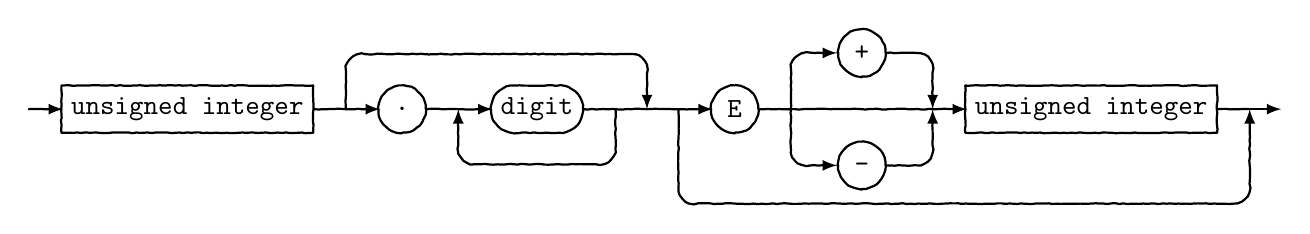
\begin{tikzpicture}[
    >=latex,thick,
    /pgf/every decoration/.style={/tikz/sharp corners},
    fuzzy/.style={decorate,
        decoration={random steps,segment length=0.5mm,amplitude=0.15pt}},
    minimum size=6mm,line join=round,line cap=round,
    terminal/.style={rectangle,draw,fill=white,fuzzy,rounded corners=3mm},
    nonterminal/.style={rectangle,draw,fill=white,fuzzy},
    node distance=4mm
  ]

    \ttfamily
    \begin{scope}[start chain,
            every node/.style={on chain},
            terminal/.append style={join=by {->,shorten >=-1pt,
                fuzzy,decoration={post length=4pt}}},
            nonterminal/.append style={join=by {->,shorten >=-1pt,
                fuzzy,decoration={post length=4pt}}},
            support/.style={coordinate,join=by fuzzy}
        ]
        \node [support]             (start)        {};
        \node [nonterminal]                        {unsigned integer};
        \node [support]             (after ui)     {};
        \node [terminal]                           {.};
        \node [support]             (after dot)    {};
        \node [terminal]                           {digit};
        \node [support]             (after digit)  {};
        \node [support]             (skip)         {};
        \node [support]             (before E)     {};
        \node [terminal]                           {E};
        \node [support]             (after E)      {};
        \node [support,xshift=5mm]  (between)      {};
        \node [support,xshift=5mm]  (before last)  {};
        \node [nonterminal]                        {unsigned integer};
        \node [support]             (after last)   {};
        \node [coordinate,join=by ->] (end)        {};
    \end{scope}
    \node (plus)  [terminal,above=of between] {+};
    \node (minus) [terminal,below=of between] {-};

    \begin{scope}[->,decoration={post length=4pt},rounded corners=2mm,
            every path/.style=fuzzy]
        \draw (after ui)    -- +(0,.7)  -| (skip);
        \draw (after digit) -- +(0,-.7) -| (after dot);
        \draw (before E)    -- +(0,-1.2) -| (after last);
        \draw (after E)     |- (plus);
        \draw (plus)        -| (before last);
        \draw (after E)     |- (minus);
        \draw (minus)       -| (before last);
    \end{scope}
\end{tikzpicture}


\begin{tikzpicture}[
        point/.style={coordinate},>=stealth',thick,draw=black!50,
        tip/.style={->,shorten >=0.007pt},every join/.style={rounded corners},
        hv path/.style={to path={-| (\tikztotarget)}},
        vh path/.style={to path={|- (\tikztotarget)}},
        text height=1.5ex,text depth=.25ex % align text horizontally
    ]
    \matrix[column sep=4mm] {
        % First row:
        & & & & & & &  & & & & \node (plus) [terminal] {+};\\
        % Second row:
        \node (p1) [point] {}; & \node (ui1) [nonterminal] {unsigned integer};&
        \node (p2) [point] {}; & \node (dot) [terminal]    {.};               &
        \node (p3) [point] {}; & \node (digit) [terminal]    {digit};         &
        \node (p4) [point] {}; & \node (p5)  [point]  {};                     &
        \node (p6) [point] {}; & \node (e)   [terminal]    {E};               &
        \node (p7) [point] {}; &                                              &
        \node (p8) [point] {}; & \node (ui2) [nonterminal] {unsigned integer};&
        \node (p9) [point] {}; & \node (p10) [point]       {};\\
        % Third row:
        & & & & & & &  & & & & \node (minus)[terminal] {-};\\
    };

    { [start chain]
        \chainin (p1);
        \chainin (ui1)   [join=by tip];
        \chainin (p2)    [join];
        \chainin (dot)   [join=by tip];
        \chainin (p3)    [join];
        \chainin (digit) [join=by tip];
        \chainin (p4)    [join];
        { [start branch=digit loop]
        \chainin (p3) [join=by {skip loop=-6mm,tip}];
        }
        \chainin (p5)    [join,join=with p2 by {skip loop=6mm,tip}];
        \chainin (p6)    [join];
        \chainin (e)     [join=by tip];
        \chainin (p7)    [join];
        { [start branch=plus]
        \chainin (plus)  [join=by {vh path,tip}];
        \chainin (p8)    [join=by {hv path,tip}];
        }
        { [start branch=minus]
        \chainin (minus) [join=by {vh path,tip}];
        \chainin (p8)    [join=by {hv path,tip}];
        }
        \chainin (p8)    [join];
        \chainin (ui2)   [join=by tip];
        \chainin (p9)    [join,join=with p6 by {skip loop=-11mm,tip}];
        \chainin (p10)   [join=by tip];
  }
\end{tikzpicture}

\end{document}